\chapter{Implementation}
\label{cha:implementation}


\section{Backend}

\subsection{Architecture}

In this section we will focus on the architecture and our decisions on backend side and its communication. We built a RESTful API which allows clients to communicate with the backend via the JSON format. The figure \ref{fig:system-overview} shows what the architecture consisted of. We had two different client applications which were communicating with the backend and a federation provider,further backend specific information about the federation provider will follow in chapter \ref{federation-provider}. The backend persisted the data into a mongoDB database. The SNET department provided us a virtual machine at the address \url{http://piazza.snet.tu-berlin.de}, where we could setup our environment.

We developed the backend with Node.JS\footnote{\url{https://nodejs.org/en/}} with the purpose that the SNET department could use or integrate it later into other projects which are mostly written in Node.JS. For our web application we used the Express web framework which influenced us in the structure of how our application is built. Our file structure consisted of five main directories:
\begin{itemize}
  \item \textbf{Controllers} are the specific implementation for an API endpoint request.
  \item \textbf{Routes} link an endpoint to a controller.
  \item \textbf{Models} are schemas for the presistent data in the database.
  \item \textbf{Middleware} takes care of our authentication.
  \item \textbf{Tests} are provided for some of the important controllers.
\end{itemize}

\subsection{Controllers}

We designed four controllers which are also part of our API endpoints to handle all requests to our API. \texttt{companionrequests} handles the creation and modification of a companion request. This means that a user wants to add a colleague to her/his friends list and she/he asks her/his friend for permission. If she/he accepts it, both parties are added to each others friends list. If she/he denies it, the requesting user will be notified about the changed status. The controller \texttt{hotspot} gives back all information about the defined hotspots like mensa or library. This includes GPS coordinates, companyUUID, major and minor of the Estimote Bluetooth Beacons contained in the area. For retrieving or modifying user specific information like her/his location, groups and settings the \texttt{users} controller is the handler for these kind of requests. The last controller is the \texttt{login} controller which on successful login returns some information about the logged in user.

\subsection{Routes}

Routes specifies a specific endpoint for a defined URI\footnote{URI=Uniform Resource Identifier}. Our routes link mostly with the same name to the controllers which we defined above. Since we have an RESTful API the expressjs framework also allows us to define GET,POST,PUT and UPDATE functionality. All endpoints are secured via our middleware which we will describe in section \ref{backend-middleware}.

\subsection{Models}
\label{mongodb-models}

Mongoose\footnote{\url{http://mongoosejs.com/}} is a powerful plugin for nodejs which allows us to have an easier connection to the mongoDB database. For this we have to define schema's for our models. So we definded four schemas companionrequest, hotspot, location and user. But not every information have to be an extra collection in the mongoDB. We definded subdocuments for those information which dont need an extra collection. For example the beacons are always in a hotspot so there is no need for an extra collection.

%define models

\subsection{Middleware}
\label{backend-middleware}

The middleware is provided by the cyclone projekt which handels the authentication and session management to the federation provider. If the user doesn't exist in our database the authentication middleware will add it with the informations which he gets from the federation provider. This includes the name, email and the ID which is also given from the authentication token of the user. We overloaded this middleware for the test section below. Which allows us to have a valid authentication against the database.

\subsection{Test}

- Server setup\\
- Docker deployment\\
- List of important API endpoints\\
- Tests

\subsection{CYCLONE Federation Provider}
\label{federation-provider}

\begin{center}
    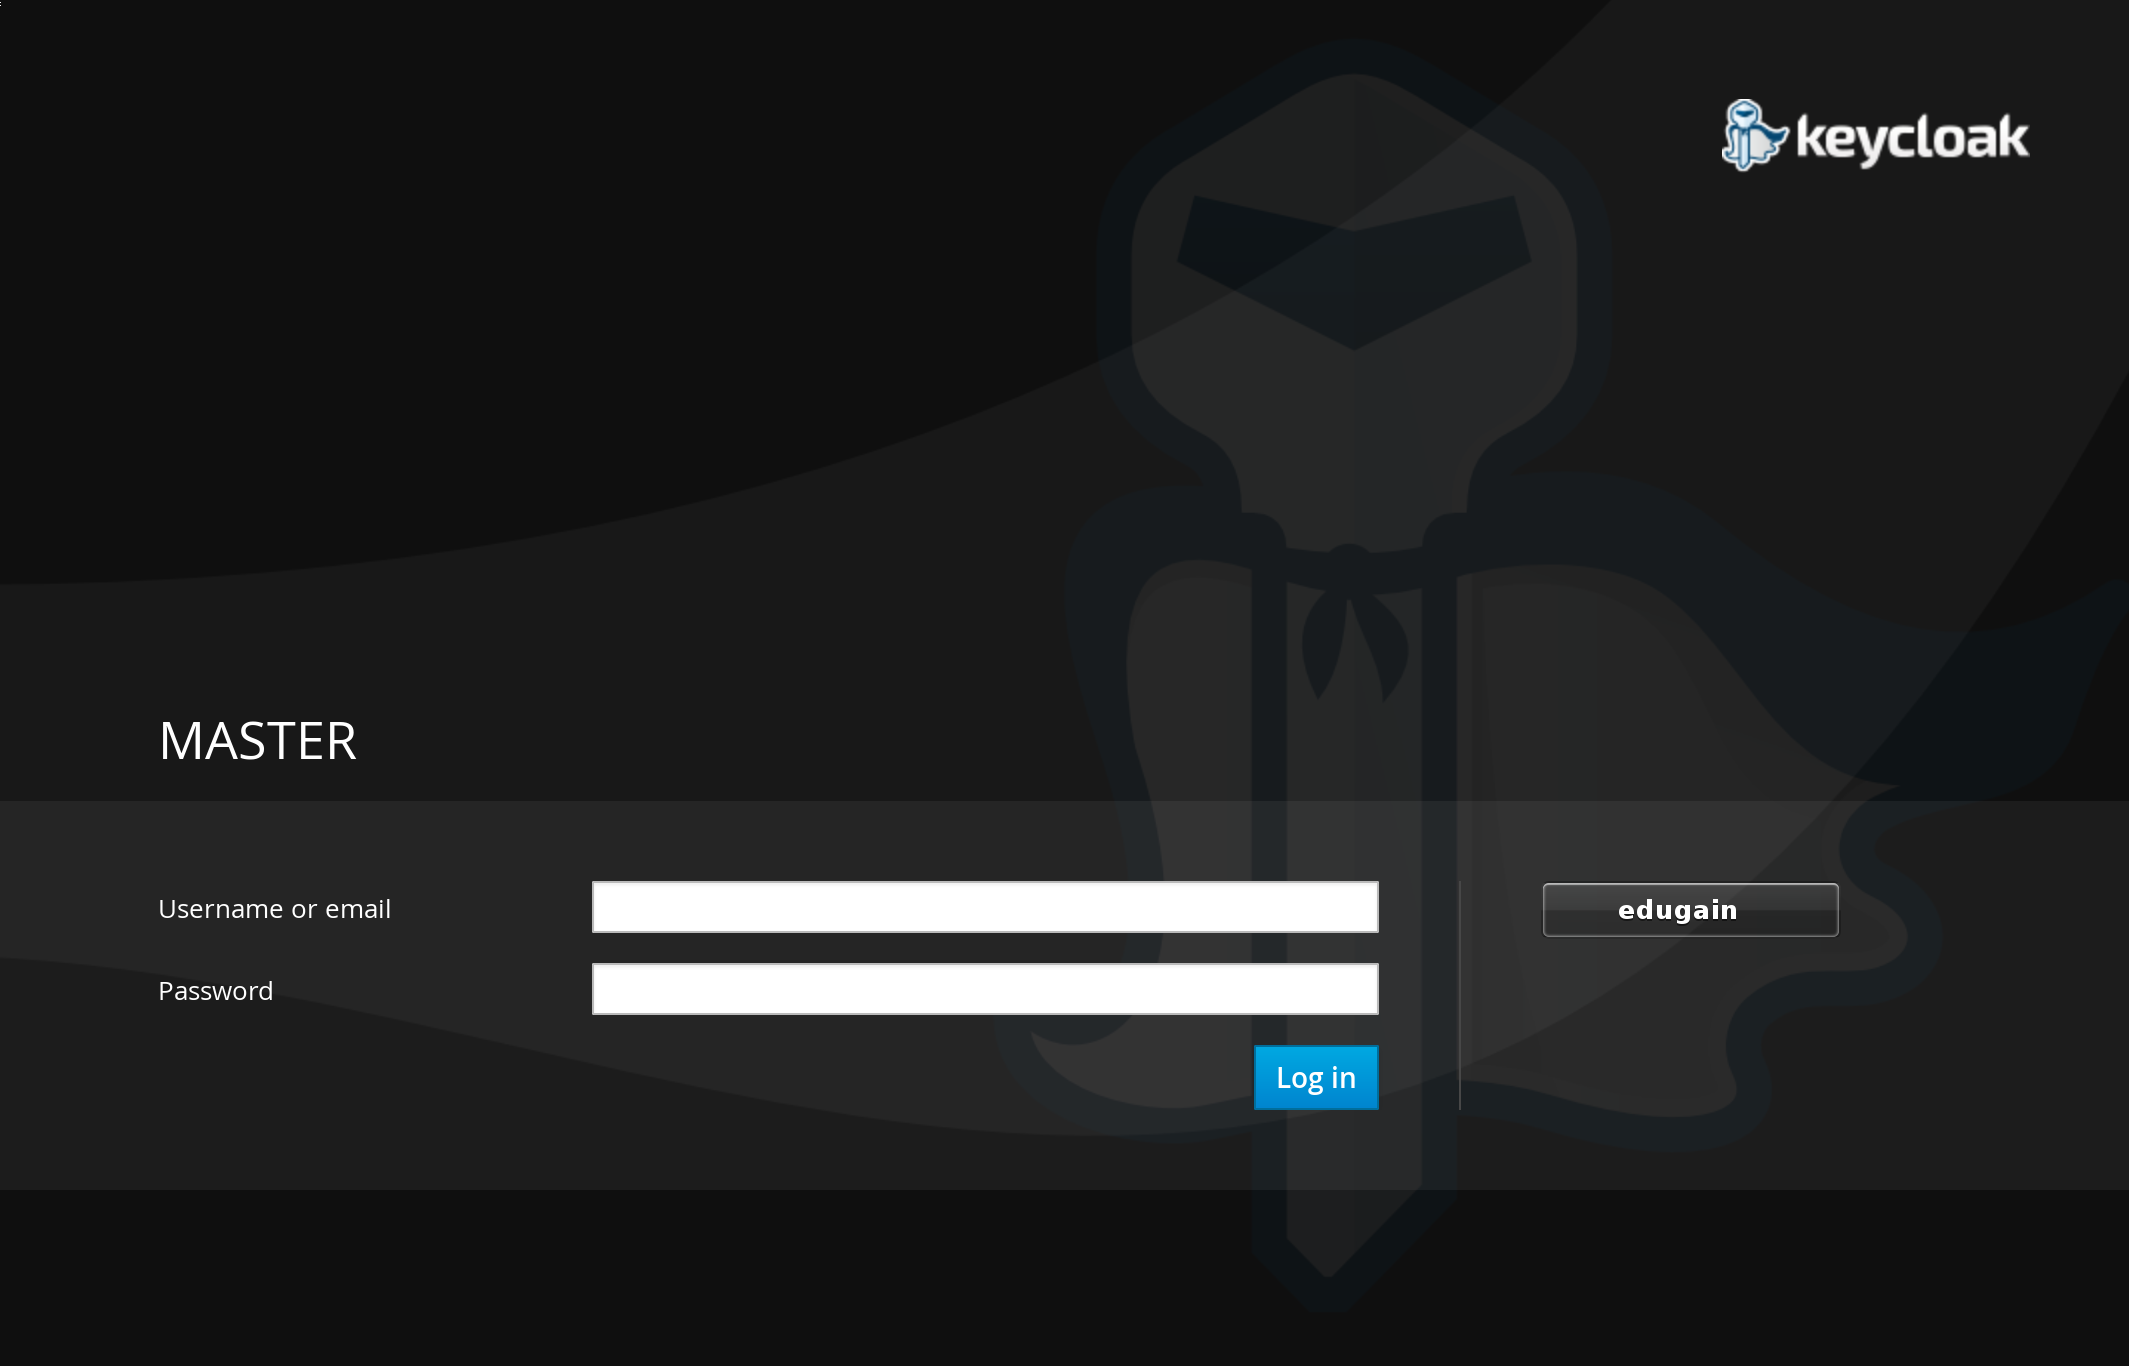
\includegraphics[width=\textwidth]{cyclone-federation-provider-login}\\
    Login screen to CYCLONE Federation Provider.
\end{center}


\vspace{0.5cm}

\section{Android}




\vspace{0.5cm}

\section{iOS}


The iOS application provides the user with a map of the specific hotspot. For this project the example of indoor navigation inside the mensa has been implemented. The app shows two floors fo the mensa, together with additional informations about the Location.

\subsection{Floorplans}
In order to show positions of the user and friends with the exact coordinates on the map, the floorplan material is added as MKOverlay on top of the MKMapView provided by Apple. We use the PDF files provided by Studentenwerk Berlin for this project. 

Apple also provides registered iOS developers with a framework to manage the mapping of x/y coordinates of the PDF file with the exact Latitude/Longitude real world coordinates of the map 
~\ref{fig:map1}.

This framework has been used for this project to integrate the floorplan of the mensa. The GeoAnchor class provided by apple converts each corner of a PDF rectangle into an MKMapPoint. The collection of MKMapPoints is combined to MKPolygon which. MKPolygons are used to draw elements and annotations on top of a map. This technology is used to divide the map in multiple maptiles that can be added to the map ~\ref{fig:map2}.


\begin{figure}
\centering
\begin{minipage}{.5\textwidth}
  \centering
  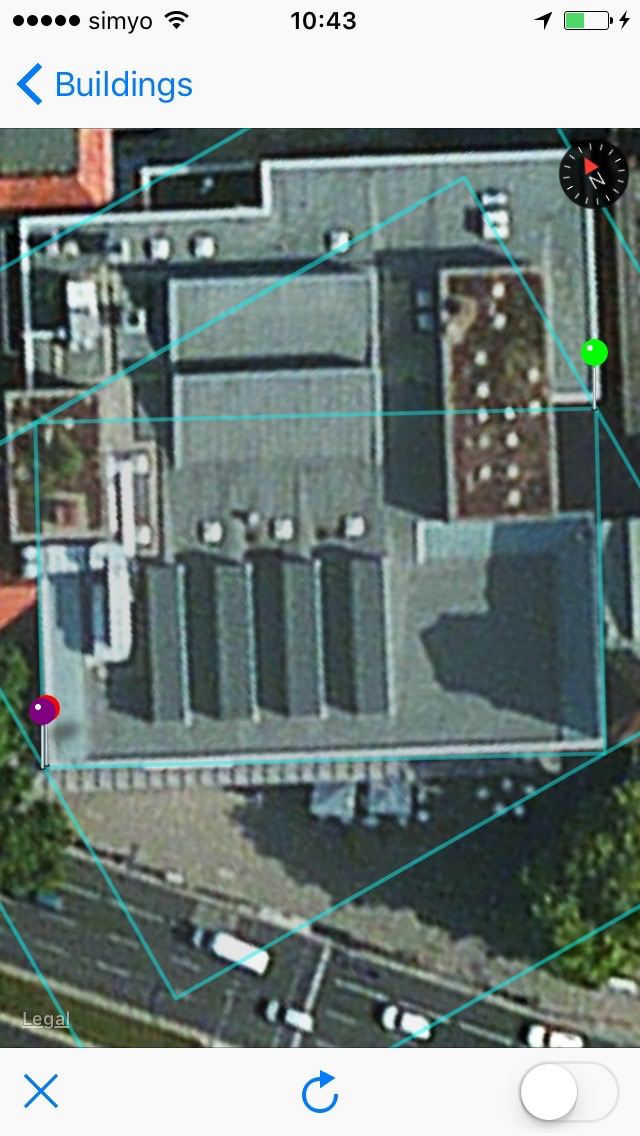
\includegraphics[width=.5\linewidth]{map1}
  \captionof{figure}{Defined Anchor Points and Boundaries}
  \label{fig:map1}
\end{minipage}%
\begin{minipage}{.5\textwidth}
  \centering
  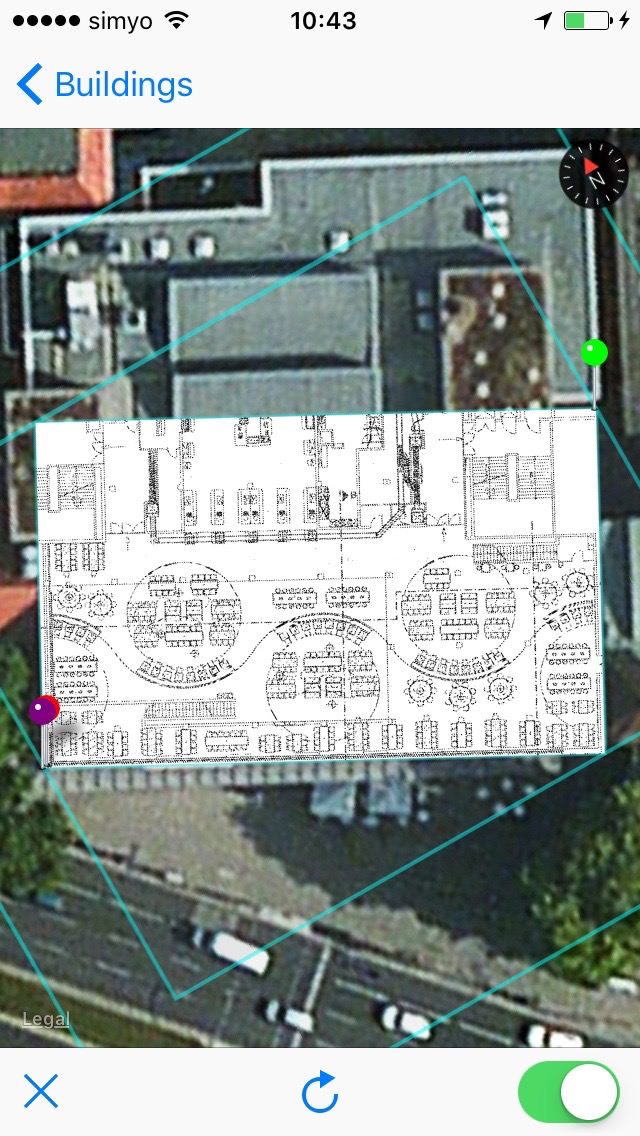
\includegraphics[width=.5\linewidth]{map2}
  \captionof{figure}{Applied Floorplan to the defined Boundaries}
  \label{fig:map2}
\end{minipage}
\end{figure}


\subsection{Login}

In order to use the application, the user has to login via Federation Provider, in order to get
a security token which grants access to the application server. \\

The app handles the login process using a UIWebView. The login request will then be redirected
to the Tubit login page ~\ref{fig:login1}, where the user finally can type in Tubit username and password.
If the user credentials are correct, the webview gets redirected to the piazza application server.

If the WebView was able to access the application server successfully, the WebView closes and grants the user access to the application. The WebView can not be bypassed without a successful login via Federation Provider ~\ref{fig:login2}. Each request to the application server reopens the WebView again, if the used security token is invalid or if the user has been logged out.


\begin{figure}
\centering
\begin{minipage}{.5\textwidth}
  \centering
  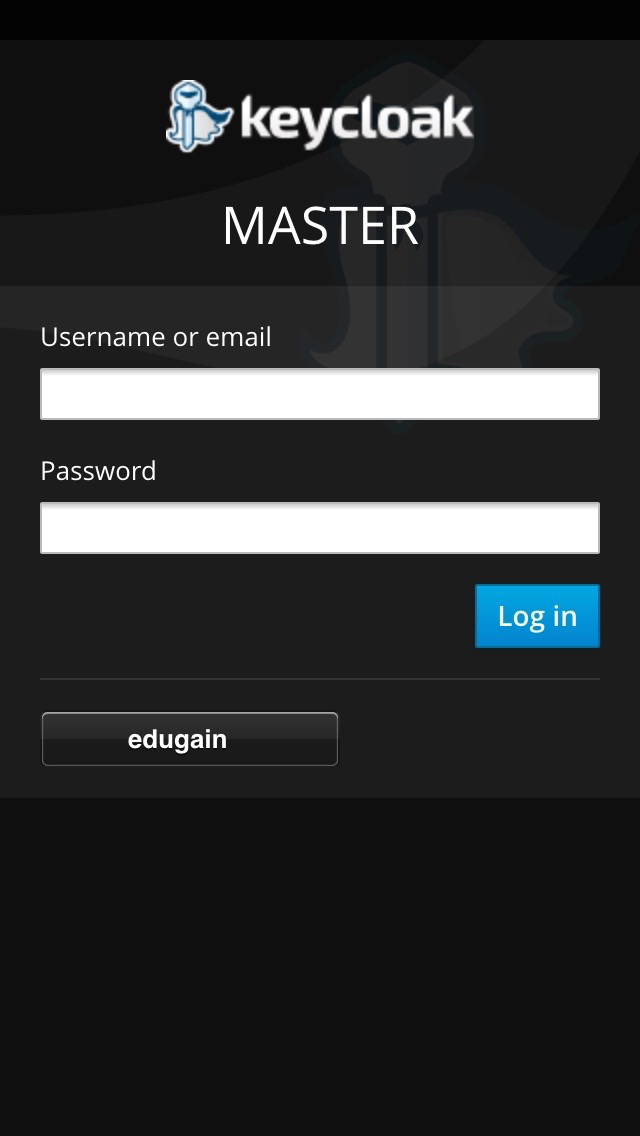
\includegraphics[width=.5\linewidth]{login1}
  \captionof{figure}{Keycloak/Federation Provider}
  \label{fig:login1}
\end{minipage}%
\begin{minipage}{.5\textwidth}
  \centering
  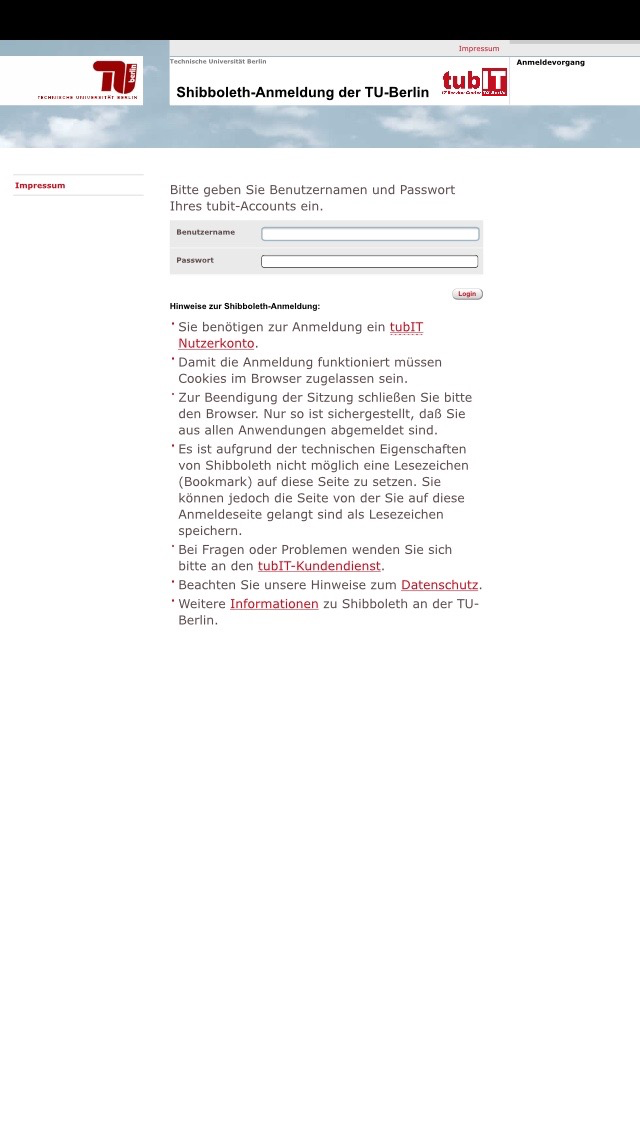
\includegraphics[width=.5\linewidth]{login2}
  \captionof{figure}{Tubit Login Page}
  \label{fig:login2}
\end{minipage}
\end{figure}

\subsection{Hotspots/ Buildings}

\begin{figure}
\centering
\begin{minipage}{.5\textwidth}
  \centering
  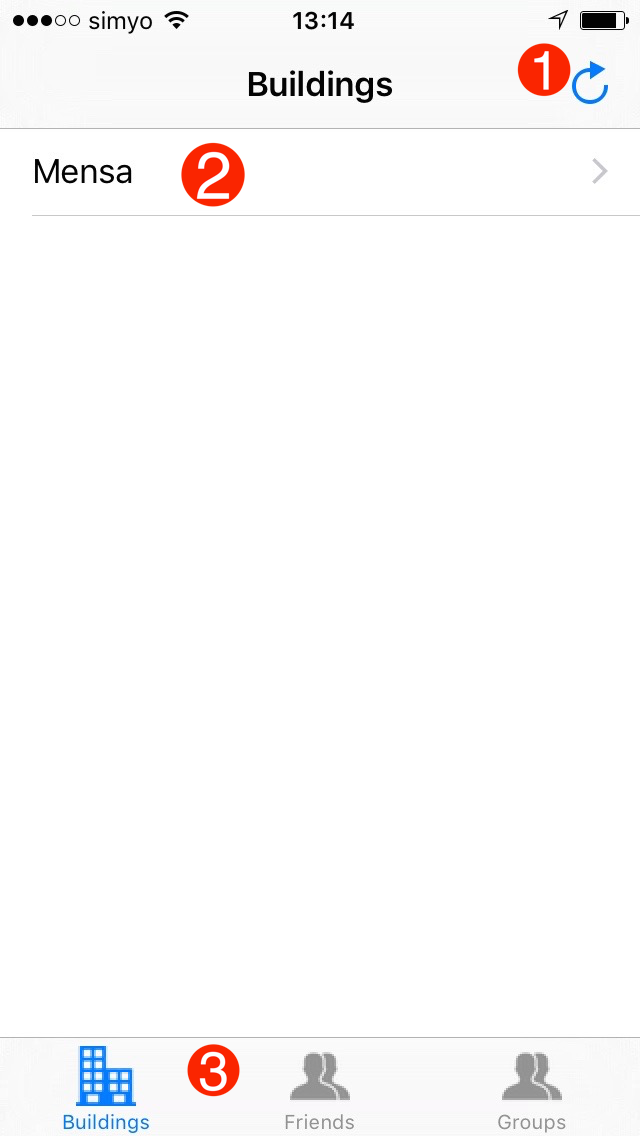
\includegraphics[width=.5\linewidth]{showbuildings}
  \captionof{figure}{List of available Hotspots}
  \label{fig:showbuildings}
\end{minipage}%
\begin{minipage}{.5\textwidth}
  \centering
  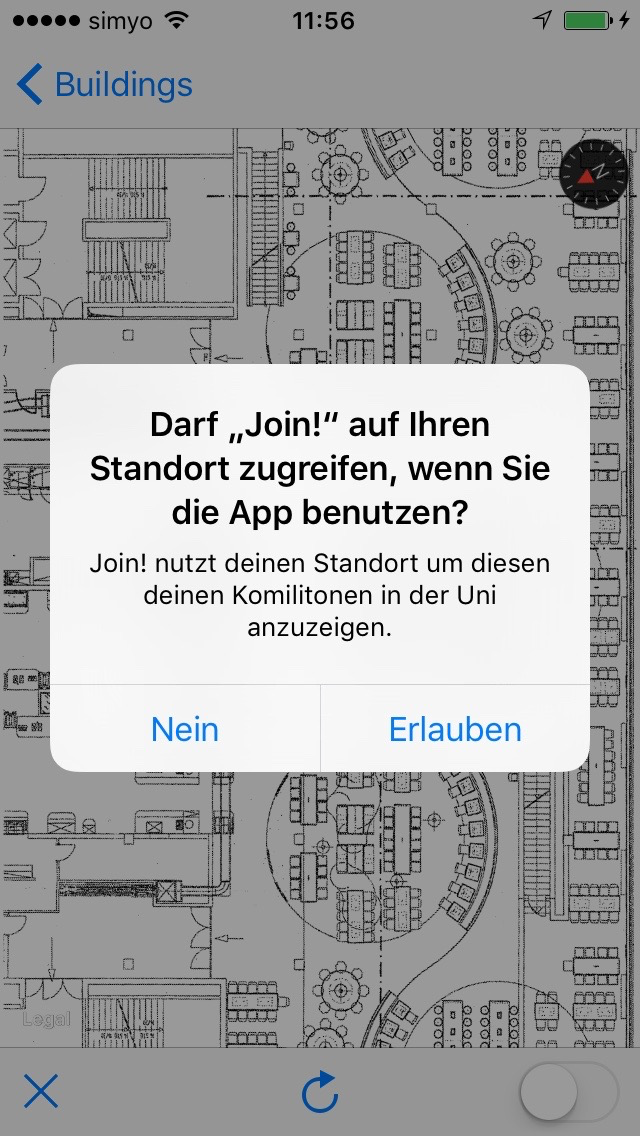
\includegraphics[width=.5\linewidth]{request1}
  \captionof{figure}{Access Location Request}
  \label{fig:request1}
\end{minipage}
\end{figure}



The Buildings View ~\ref{fig:showbuildings} is the first view the user sees after login. This view enlists all available Hotspots delivered by the Backend.

\begin{enumerate}
  \item The reload button, calls the Backend to get a list of available hotspots. The list contains the hotspots and the available beacon and floor information.
  \item The Tableview lists all available hotspots from the Backend. Each cell contains the name of a Hotspot.
  \item The Application is divided into three contextual distinct parts: Buildings, Friends and Groups. This subdivision is implemented in a UITabBar which is the leading element of the application architecture.
\end{enumerate}

\subsection{Indoor Positioning}

\begin{figure}
\centering
\begin{minipage}{.5\textwidth}
  \centering
  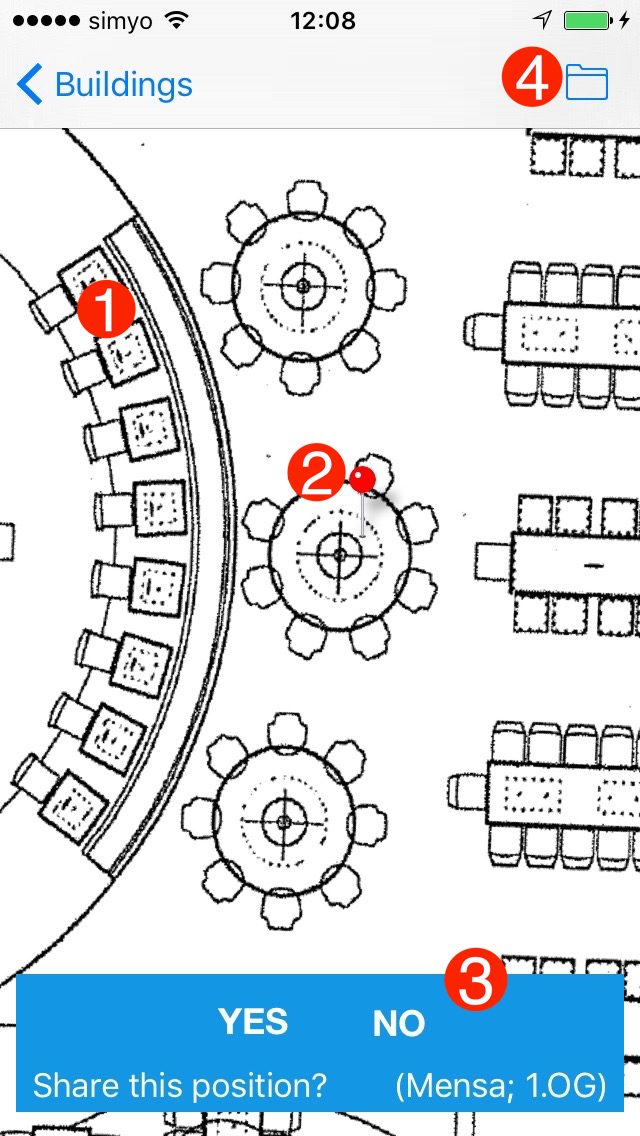
\includegraphics[width=.5\linewidth]{shareposition}
  \captionof{figure}{Share Position Mode}
  \label{fig:shareposition}
\end{minipage}%
\begin{minipage}{.5\textwidth}
  \centering
  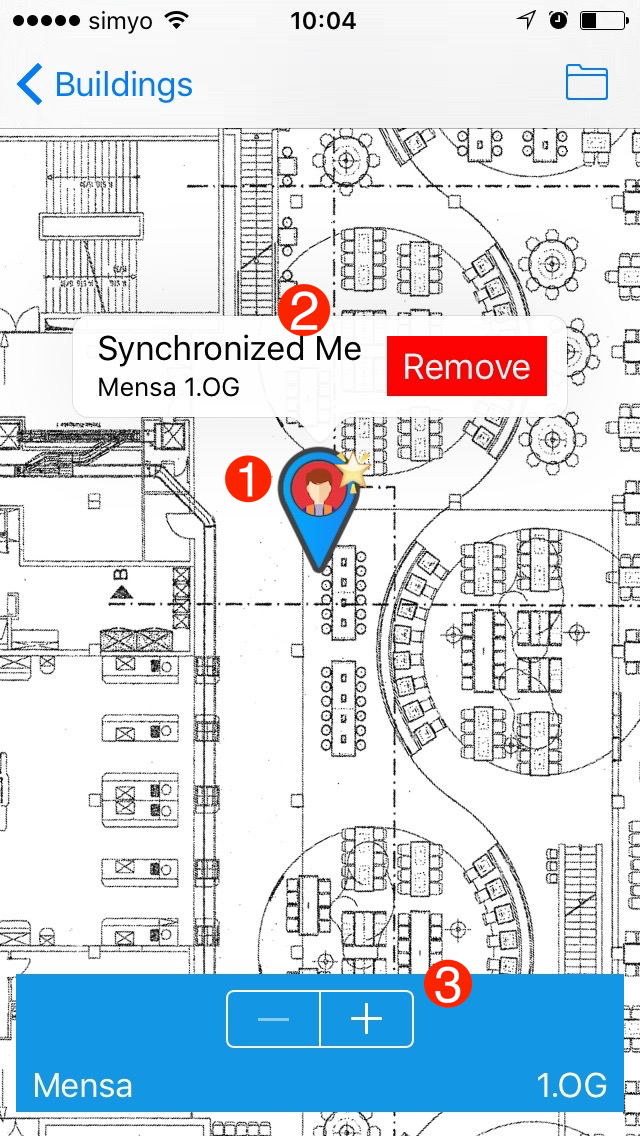
\includegraphics[width=.5\linewidth]{synchronizedme}
  \captionof{figure}{Synchronized Position Mode}
  \label{fig:synchronizedme}
\end{minipage}
\end{figure}


If the user taps on one of the Buildings enlisted in the Buildings View, the app opens respectively
the coresponding floorplan in an MKMapView. Figure ~\ref{fig:shareposition} shows the mensa floorplan on a large scale. This functionality was added additionaly in order to increase the usability and accuracy of manual pin-pointing.

\begin{enumerate}
\item The the MapView shows the first floor of the mensa by default, if the Tubit-MSE api which provides the floor and building information is not available. In cases of availability of the Tubit-MSE api, the MapView shows the corresponding floor as soon as the MapView appears on the screen.

\item The manual pin pointing of the users position is triggered by a so called long press on the map which was additionally implemented. The long press is a distinct user-interaction mode. It is applied as solution for manual pin pointing on iOS in order to prevent the user from mistakenly share  positions by inadvertently touching the map. After a long press is registered by the system, it drops a red pin on the position where the user pressed. This switches the MapView into a share position mode. In this mode the user can touch on any place on the map to easily edit or remove the pin, if the position to share is not correct.

\item The information panel is used to give the user the posibility to change the floor by pushing the plus (up) or minus(down) buttons. The Informationpanel also flips with an animation, signaling the user of the changed mode of the MapView. The flip animation is triggered as soon as the system successfully registeres a long press. In Share Position Mode the Information-Panel prompts the user to share the location.

\item The File-Button modally opens a settings view.
\end{enumerate}


Figure ~\ref{fig:synchronizedme} shows the MapView after a user has successfully share the position either via Bluetooth Beacon, automatically using the Apple CLLocation Framework or manually via pin-pointing.


\begin{enumerate}
\item As soon as the backend has received the new location of the user successfully, the red pin is exchanged with a marker annotation. This marker shows the provided synchronized location of the user. The switch of the marker gives the user a hint, that his position is now synchronized with the server state. This marker is also used for the positions of friends, however the user position is highlighted with a star.
\item If the user taps on his own marker, it reweals an annotation view that includes the user name as well as a remove button that deletes the shared position from the server permanently.

\item The Information-Panel is now flipped back to Normal mode or Synchronized Position Mode if the user previously shared the position manually.
\end{enumerate}


The Settings view (see Figure ~\ref{fig:settings1} and ~\ref{fig:settings2}) provides additional options to indoor positioning and Information Annotations that are shown on the floorplan.

\begin{figure}
\centering
\begin{minipage}{.5\textwidth}
  \centering
  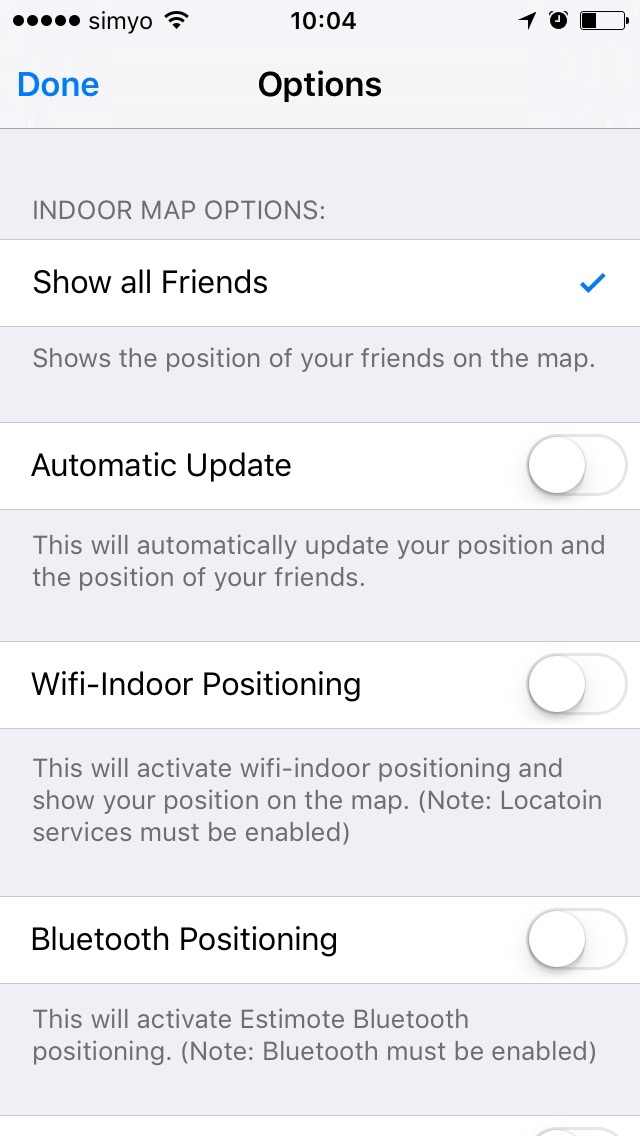
\includegraphics[width=.5\linewidth]{settings1}
  \captionof{figure}{Map Settings 1}
  \label{fig:settings1}
\end{minipage}%
\begin{minipage}{.5\textwidth}
  \centering
  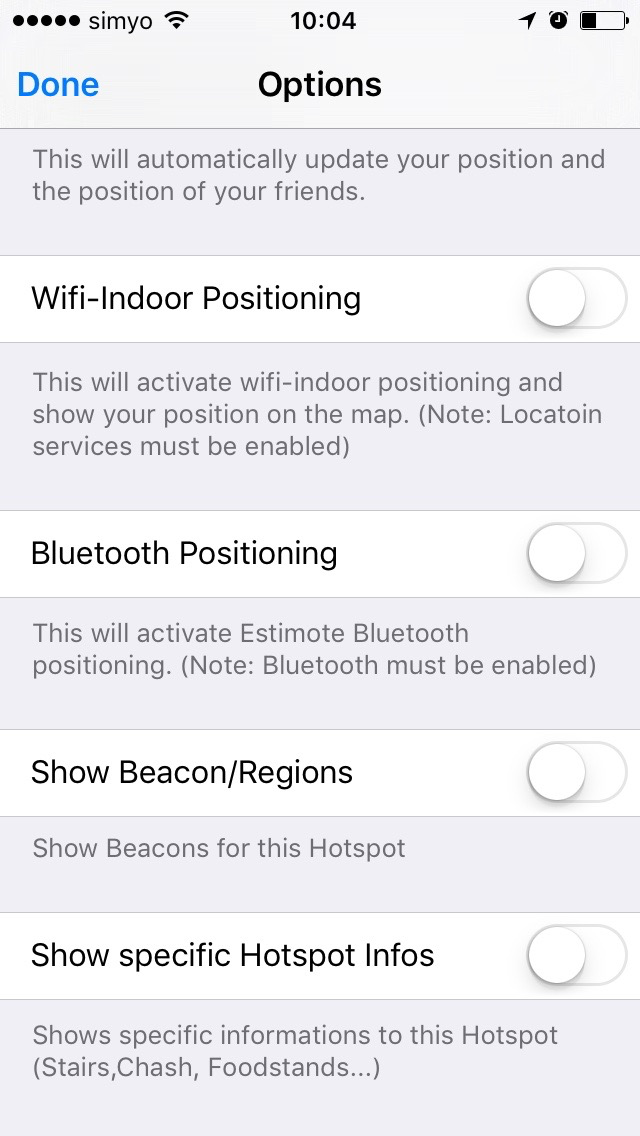
\includegraphics[width=.5\linewidth]{settings2}
  \captionof{figure}{Map Settings 2}
  \label{fig:settings2}
\end{minipage}
\end{figure}

\begin{enumerate}
\item \textbf{Show all Friends} activates annotations for Friends in the same hotspot. (Note: Friends will only be shown on the map if the user has shared his own position before)
\item \textbf{Automatic Update} activates a routine that constantly requests the server for location updates of friends. 
\item \textbf{Wi-Fi Indoor-Positioning} activates the CLLocation positioning. This will automatically update the user position while moving through the Building.
\item \textbf{Bluetooth-Positioning} activates location sharing via bluetooth beacons
\item \textbf{Show Beacons/Regions} activates annotations showing Beacons placed in the Hotspot
\item \textbf{Show Specific Hotspot Informations} activates annotations showing specific hotspot informations.
\end{enumerate}

If the user activates \textbf{Show all Friends} on settings and has already shared the own position, the mapview adds Markers for each friend located in the same hotspot. The friend markers are equipped with Accuracy-Circles placed underneath the marker. The radius of the Accuracy-Circles decreases with the accuracy of the shared position. If a position is manually shared, no Accuracy-Circle will be shown. However, if the position is shared via Bluetooth or Wi-Fi, the Accuracy-Circle increases to show the region the friends position (see Figure ~\ref{fig:showfriends}). 

If the user activates \textbf{Show Specific Hotspot Informations} on settings, the MapView will show the user specific Informations regarding the Hotspot such as Cashregister or Foodstands. This functionality has been added in order to improve the usability of the Floorplan and helps the user to orientate in the building (see Figure ~\ref{fig:additionalinfo}).

\begin{figure}
\centering
\begin{minipage}{.5\textwidth}
  \centering
  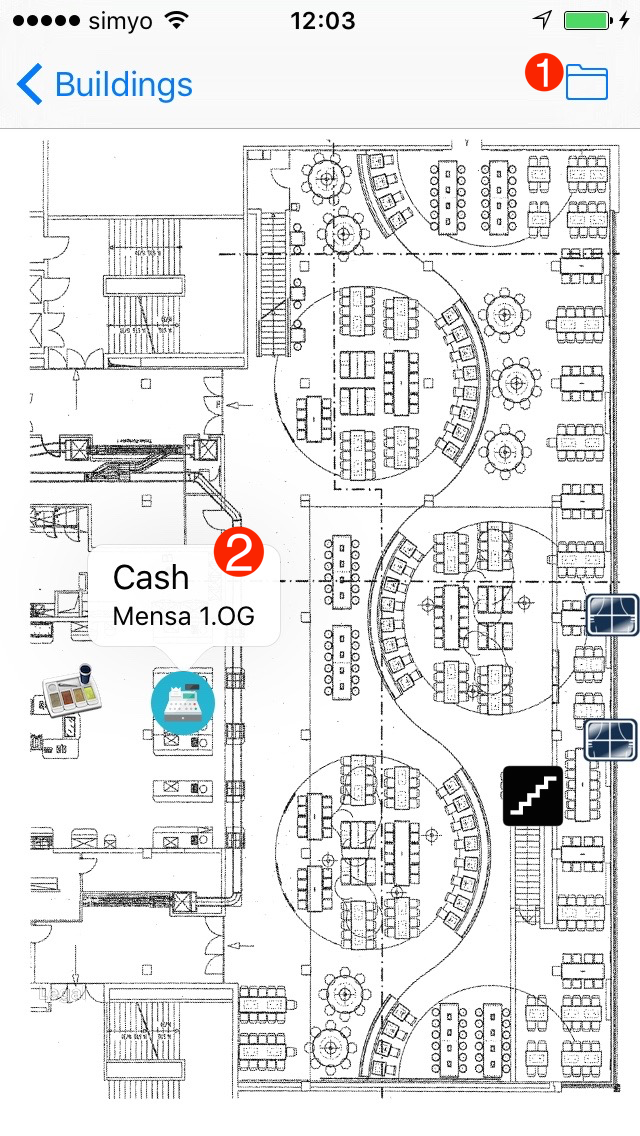
\includegraphics[width=.5\linewidth]{additionalinfo}
  \captionof{figure}{Additional Hotspot Informations}
  \label{fig:additionalinfo}
\end{minipage}%
\begin{minipage}{.5\textwidth}
  \centering
  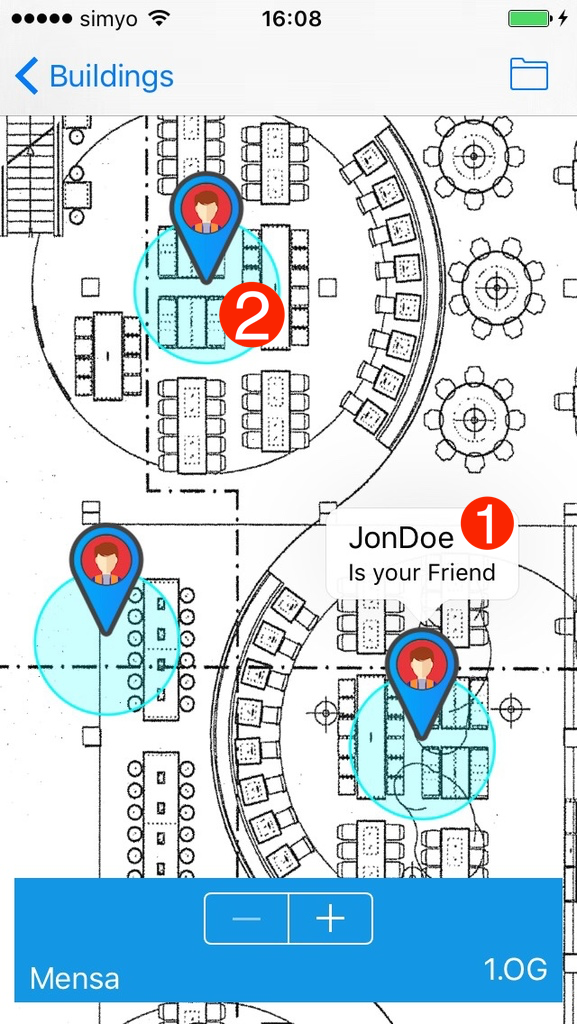
\includegraphics[width=.5\linewidth]{showfriends}
  \captionof{figure}{Friends in this Hotspot with Accuracy}
  \label{fig:showfriends}
\end{minipage}
\end{figure}


\subsection{Friends}

As soon as the user tabs on the All Friends button of the TabBar, the application shows the All my Friends List ~\ref{fig:friendlist}. This View shows either the friends of the user or opens companion requests that the user needs to accept in order to add a person into his friends list. Note that all available friends will be shown in this list regardless of their group affiliation.

\begin{figure}
\centering
\begin{minipage}{.5\textwidth}
  \centering
  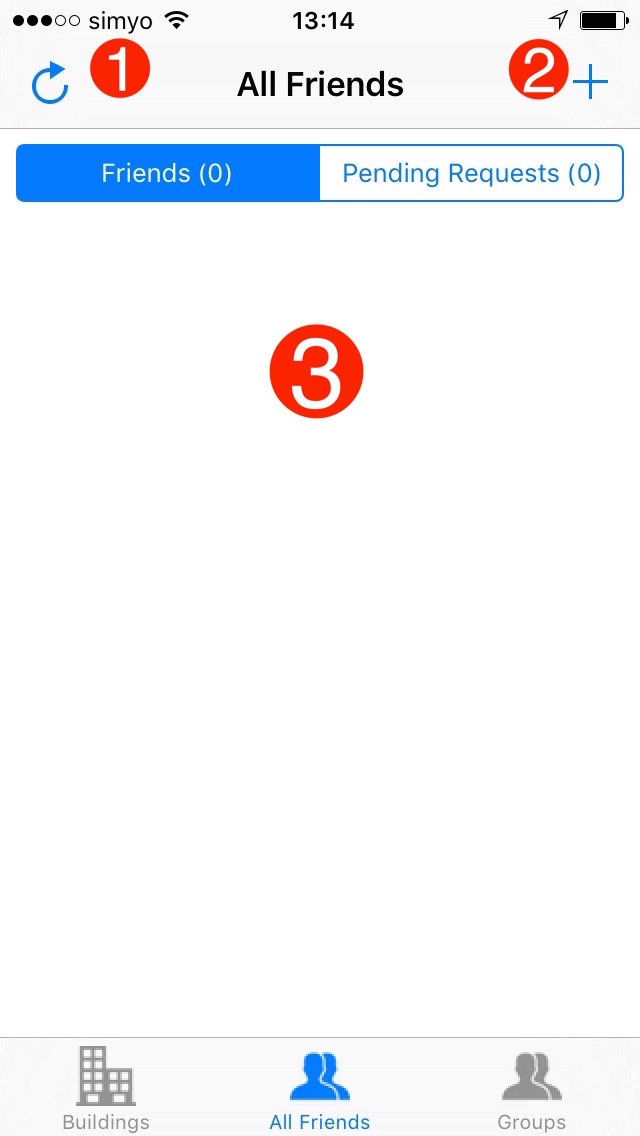
\includegraphics[width=.5\linewidth]{friendlist}
  \captionof{figure}{Available Friends and Open Requests}
  \label{fig:friendlist}
\end{minipage}%
\begin{minipage}{.5\textwidth}
  \centering
  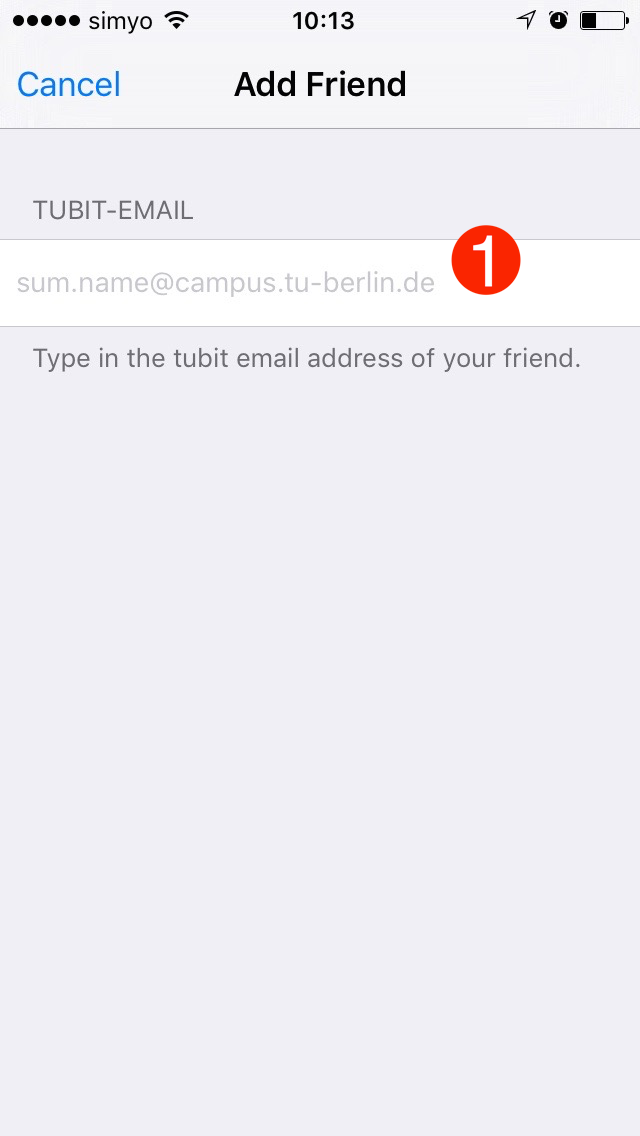
\includegraphics[width=.5\linewidth]{addfriend}
  \captionof{figure}{Add Friends}
  \label{fig:addfriend}
\end{minipage}
\end{figure}

\begin{enumerate}
\item The Reloadbutton is implemented in order to update the list of friends or new companion requests. In future work the server should be able to send remote notifications in order to inform the user of new companion requests.

\item The Plus button is implemented to open a new view ~\ref{fig:addfriend} where the user can add new friends and send new companion requests.

\item The list view is managed by a UISegmentControl. The content is divided into available friends and available Companionrequests. These are shown by numbers. A tap on one of the segments will either change the content of the TableView to friends or companion requests. The entry of the list contains the provided name of a friend.
\end{enumerate}


As seen on ~\ref{fig:addfriend}, the app opens modally a new view that enables the user to add new friends.

\begin{enumerate}
\item The UITextfield is used in order to enable the user to type in the email address of a friend. This request will be handed by the backend. The response of the backend about the success or fail of the request will be directly shown under the textfield.
\end{enumerate}

\subsection{Groups}

\begin{figure}
\centering
\begin{minipage}{.5\textwidth}
  \centering
  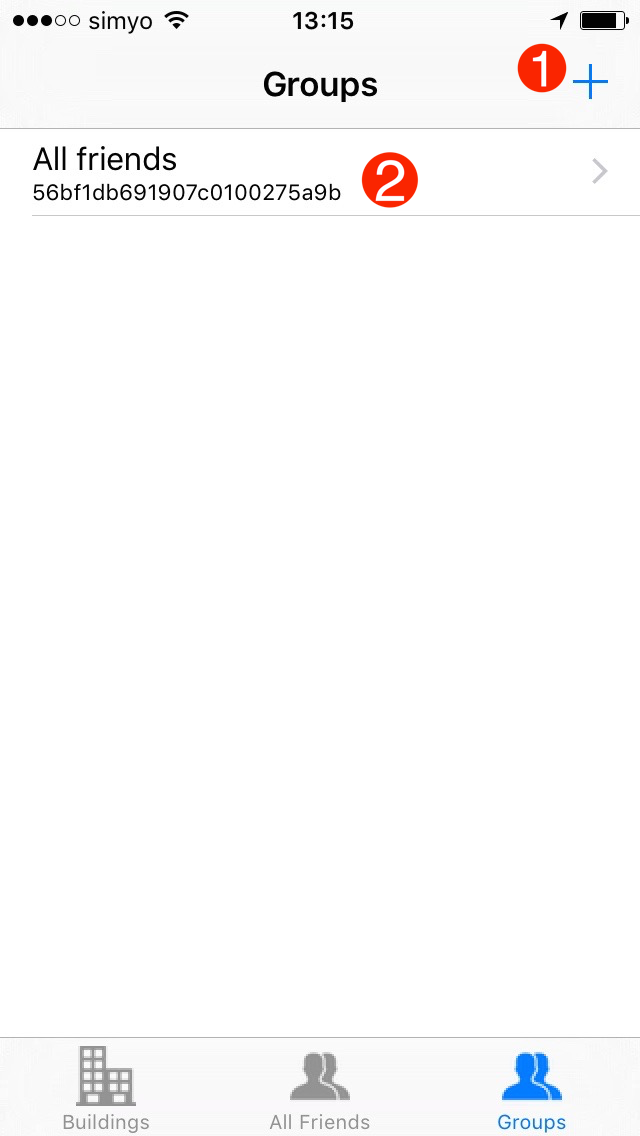
\includegraphics[width=.5\linewidth]{showgroups}
  \captionof{figure}{Show available groups}
  \label{fig:showgroups}
\end{minipage}%
\begin{minipage}{.5\textwidth}
  \centering
  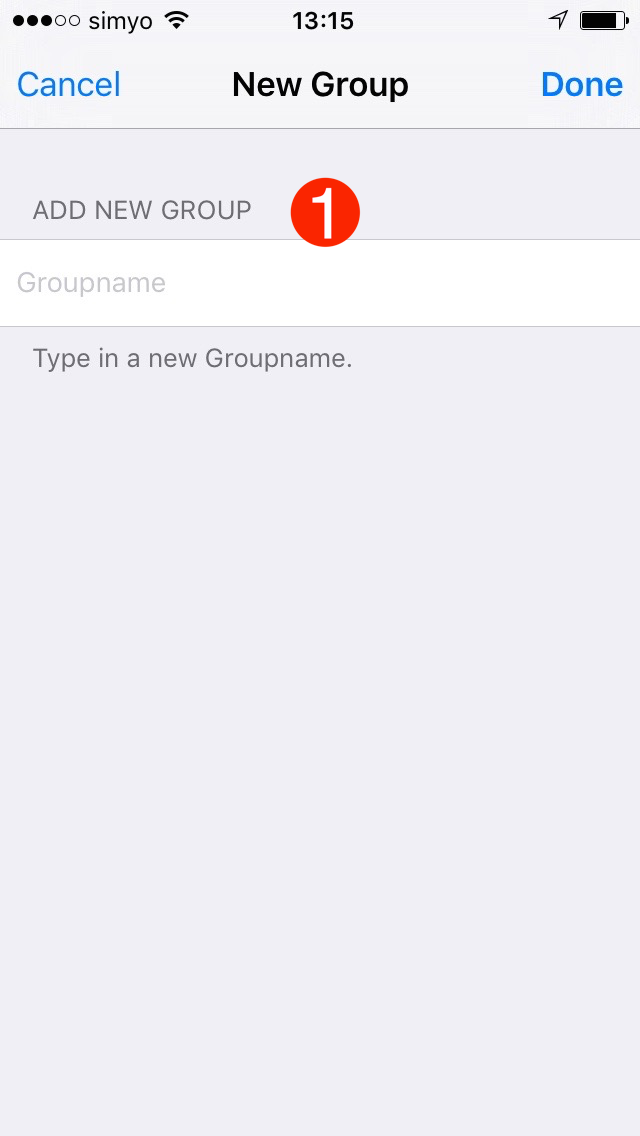
\includegraphics[width=.5\linewidth]{addgroup}
  \captionof{figure}{Add new group}
  \label{fig:addgroup}
\end{minipage}
\end{figure}

The backend enables the user to manage groups. Each user has a group named All friends, containing all of the users friends. Additionally the user may have different friends that can be added to own groups. These groups will be enlisted in this Table View as shown in ~\ref{fig:showgroups}. 

\begin{enumerate}
 \item The plus-button will open a new view modally that enables the user to create a new group (see ~\ref{fig:addgroup}).
 \item This tableview shows all available groups of the user. Each cell contains of the Name of the group together with the GroupID as subtitle. For future work if the user taps a group, it will open a new list showing the members of this group. The user should also be able to add specific friends to a group as well as edit or delete a group.
\end{enumerate} 

\subsection{Geofencing}
The iOS client supports Geofencing abilities for registered Hotspots. Geofencing notifies the app when its device enters or leaves the geographical region of a Hotspot. For this project the triggered notification greats the user and acts as a reminder to use the app if the user enters the mensa. The notification can also be used to take the user in charge of the decision wether he wants to download updates about the hotspot. The notification will also act as a reminder to deactivate bluetooth if the user leaves the mensa.


\subsection{Future Work on iOS}
The iOS client build for the project shows a propper solution of mobile indoor navigation backed with a scalable backend system. However some functionalities may be added to the client as they have been out of scope of this project.

\begin{description}
  \item[Remote Notifications] \hfill \\
  Remote notification handling is state of the art in mobile applications of these days. It should be considered to equip the backend with the ability to notify a user if one of his friends shared his position in a specific hotspot, instead of constantly polling for updates. Remote Notifications would also be used to notify the user for new companion requests. Also sheduled polling for Hotspot updates is not a best practice and should be exchanged by a publish-subscribe pattern.
  \item[CLLocation Framework] \hfill \\
  In future work, the new CLLocation framework should be considered as first pick technology for indoor navigation for iOS. Authorities of locations that are interested in indoor navigation on iOS should consider an enrollment on Apples Map Connect program. With an successfull enrollment, Floor informations as well as the accuracy of the users position would be improved.
  \item[Friends/Group Management] \hfill \\
  In future work, the client should give the user more posibilities to manage his friends as moving friends to specific groups or edit groups. The map should also be equipped with the posibilities to show specific groups instead of only all friends in a building.
  
\end{description}